\section{System Architecture}
Our converting pipeline is subdivided into three main states: the \textbf{Import 
Module}, the \textbf{Canonical Scene Representation} and the \textbf{Conversion 
Module}, as illustrated in Figure \ref{fig:sysarch}. Given an arbitrary input 
file format, our converter is able to import the scene and transform it into a 
generic, canonical representation and then export it to different output 
formats. 

\begin{figure}[h]
\centering
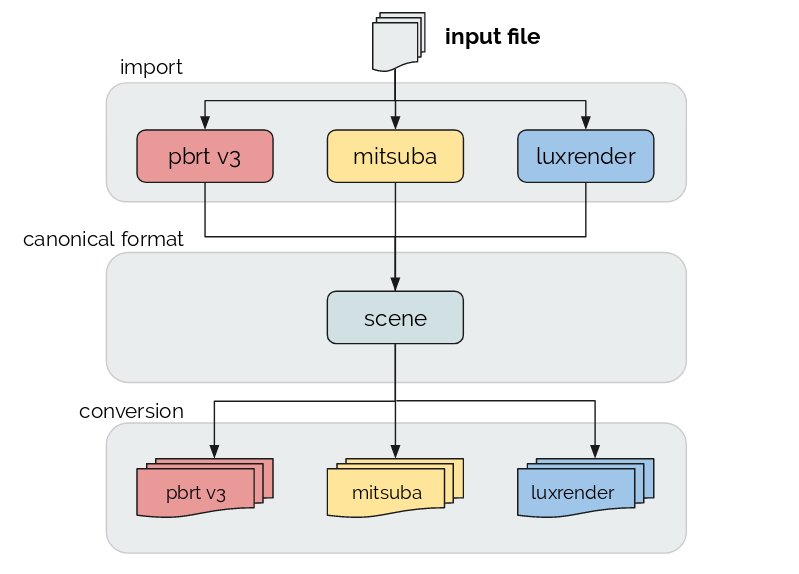
\includegraphics[width=2.5in]{figs/3_system_architecture/architecture.png}
\caption{Illustration of the system pipeline.}
\label{fig:sysarch}
\end{figure}

Our Proof of Concept encompassed \textit{PBRT} \cite{pbrt}, \textit{Mitsuba} 
\cite{mitsuba} and \textit{LuxRender} \cite{luxrender}, as these are three of 
the most popularly used renderers in the community.

\subsection{Import Module}
Most physically-based renderers have a similar way of describing a scene. 
Usually, they divide a scene into two sections: scene-wide rendering options and 
world block. The former defines overall rendering settings (such as which 
rendering or sampling technique should be used) while the latter describes the 
geometry and which materials should be used for rendering.

Our import module specializes in reading and interpreting such scene files. The 
input file is read, parsed and each directive is loaded into our canonical scene 
representation. Since each renderer has its own proprietary file format, we have 
three importing modules: one for each renderer.

\textit{PBRT} and \textit{LuxRender} file formats are composed of structured 
text statements defining all scene directives. Given their structure, a Lex/Yacc 
parser was considered the best choice for these formats. As we intended to keep 
our system in pure Python, we chose to use PLY \cite{ply}, a Python 
implementation of Lex and Yacc.

\textit{Mitsuba}'s file format consists of a XML file. Since there are several 
XML-parsing libraries for Python that can load the hierarchy into a tree data 
structure, we didn't think it necessary to create a Lex/Yacc parser. We chose to 
implement this module using ElementTree \cite{ET}, a XML parsing tool.

\subsection{Canonical Scene Representation}
After loading the scene file, the information obtained from them has to be 
stored somewhere. While most renderers have the same base structure, they differ 
in which parameters can be used to configure the techniques used during the 
rendering process. 

Renderer directives are usually given in the format of a command, followed by a 
type and a list of additional parameters. So, for instance, to specify the path 
integration technique with 8192 samples per pixel in \textit{PBRT} one would 
write the following directive: \textit{Integrator ``path'' ``integer 
pixelsamples'' [8192]}.

In order to establish a common ground for conversion, we 
defined a canonical scene representation. This representation can be easily 
extended incorporate any directives not contemplated in this work.

In this representation, we divide the scene into \textbf{scene-wide rendering 
options} and \textbf{world block}. The rendering options are divided into 
integration technique and sensor options, while the world block is divided into 
lists of shapes, global emitters and material definitions. This structure is 
illustrated in Figure \ref{fig:canonicalrep}.

\begin{figure}[h]
\centering
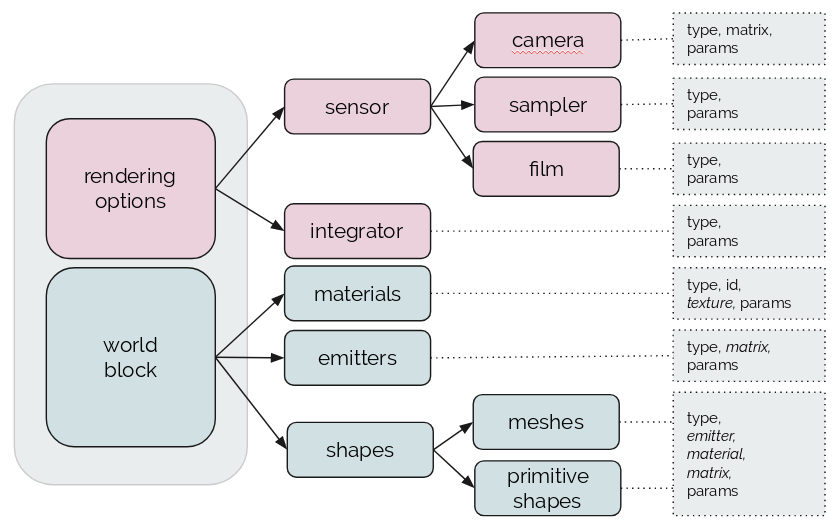
\includegraphics[width=2.5in]{figs/3_system_architecture/canonicalrep.png}
\caption{Illustration of the canonical scene representation.}
\label{fig:canonicalrep}
\end{figure}

\subsubsection{Scene-wide Rendering Options}
A set of directives specifying the integration and sampling techniques used for 
rendering, camera and film properties. These directives are represented in a 
structure with two fields: a type and a list of parameters.

\subsubsection{World Block}
A set of directives describing the shapes, materials and global emitters present 
in the scene. 

The \textbf{shape} directive is represented in a structure with: a type (cube, 
sphere, ...), an optional area emitter, an optional material reference, an 
optional transformation matrix and a list of parameters. 

The \textbf{material} directive is represented in a structure with: a type, an 
id, an optional texture and a list of parameters.

The \textbf{texture} directive is represented in a structure with: a type, an id 
and a list of parameters.

The \textbf{global emitter} directive is represented in a structure with: a 
type, an optional transformation matrix and a list of parameters.

\subsection{Conversion Module}
Subsection text here.